\chapter[Appendices] {Appendices}
\label{Appendix}

\section{Thesis website}
\label{Appendix: Thesis website}
The ongoing developments of this thesis research and a gallery of moving Semantic Form models are available on the following website: 

\url{https://orusmateo.com/thesis-what-may-be-known-2025}

\section{LaTeX manuscript repository}
\label{LaTeX GitHub}
The following web page provides access to the LaTeX code used to compile this thesis, including all figures and formatting details:

\url{https://github.com/orusmateo/Orus-MA-Thesis}

\section{Moving and interactive models}
The following web page provides access to the moving and interactive models which I developed for my thesis. 

\url{https://orusmateo.com/moving-semantic-forms}

\section{Semantic Forms surface and volume equations }
\label{Semantic Forms equations}
The following table shows the volume and surface equations of the Semantic Forms' core geometries. 
\begin{table}[h]
    \centering
    \begin{tabular}{|l|l|l|}
\hline
 & \textit{Volume (V)} & \textit{Surface (S)} \\[10pt]
 \hline
cone &  $\pi r^2 \frac{h}{3}$ & $\pi r \sqrt{r^2+h^2}$  \\[10pt] \hline
 cylinder & $\pi r^2 h$ & $2 \pi r h$ \\[10pt]
  \hline
sphere & $\frac{4}{3} \pi  R^3$ & $4 \pi r^2$ \\[10pt] \hline
horn torus & $2 \pi^2 a^3$ & $4 \pi^2 a^2$ \\[10pt] \hline
ring torus & $\frac{1}{4} \pi^2(R+r)(R-r) a^*$ & $\pi^2 (R+r)(R-r)$ \\[10pt]
\hline
\multicolumn{3}{l}

    \end{tabular}
    %\caption{Caption}
\end{table}

\begin{quote}
    \centering *Pappus’s centroid theorem \citep{weisstein_torus_nodate}.
\end{quote}

\index[people]{Pappus}
\clearpage

\section{Application of Sarajlić et al. configurations to three-dimensional graphlets}
As part of my style guide for Query Isomorphs analysis, I propose that the Sarajlić et al. graphlet configurations \citep[p. 3]{sarajlic_graphlet-based_2016} can be used for graph input and graph analysis.

\begin{figure}[h!]
    \centering
    \includegraphics[width=0.8\textwidth]{figures/5.6.png}
    \caption[Example Query Isomorph in two dimensions and three dimensions assembled from directed graphlets]{\textbf{Example Query Isomorph in two dimensions and three dimensions assembled from directed graphlets.} \\
(a) From Sarajlić et al. 2016’s point b, “Illustration of how directed graphlets assemble together to form complex networks”, from “Figure 1. Illustration of directed graphlets” \citep[p. 3]{sarajlic_graphlet-based_2016}. In keeping with Sarajlić et al., the whole network can be created by adding graphlets G4, G1, and G3, meaning that in the process, a new graphlet, G2, was created. The colours red, green, blue, and black are sourced from \citep[p. 3]{sarajlic_graphlet-based_2016}. (b) Spatial arrangement adds the semantic affordance of verticality to communicate hierarchy of the blue node. Red nodes are querying for nodes in both higher and lateral hierarchies. (c) Other arrangements can easily facilitate different relationships in the Query Isomorph. (b) and (c) The colours red, green, and blue are sourced from \citep[p. 3]{sarajlic_graphlet-based_2016} here also, but white is used instead of black for contrast. Black nodes in this example are all placed in a lateral level of hierarchy. In a functional Query Isomorph platform, nodes could also be placed higher or lower than each other. Furthermore, the angles and directions of these graphlets are presented for simplicity of the variety they can have but do not represent the diversity of angles and forms that graphlets can be configured in as Query Isomorphs. 
}
    \label{f5.6}
\end{figure}
\clearpage


\section{The Semantic Forms located in Bertin’s taxonomy of network graphs}
\begin{figure}[h!]
    \centering
    \includegraphics[width=0.9\textwidth]{figures/A.3.png}
    \caption[Groups of imposition and types of imposition]{\textbf{Groups of imposition and types of imposition} \citep[p. 52]{bertin_semiology_2011}.
From \textit{Semiology of Graphics: Diagrams, Networks, Maps} by Jacques Bertin, translated by William J. Berg. Reprinted by permission of the University of Wisconsin Press. © 1983 by the Board of Regents of the University of Wisconsin System. All rights reserved.}
    \label{fig:A3}
\end{figure}
\index[people]{Bertin, Jacques}
\index[people]{Berg, William J.}
%\clearpage
\begin{figure}[h!]
    \centering
    \includegraphics[width=\textwidth]{figures/A.4.png}
    \caption[Groups of imposition and types of imposition as categories for my Semantic Shapes, Semantic Forms, and three-dimensional gigamaps]{\textbf{Groups of imposition and types of imposition as categories for my Semantic Shapes, Semantic Forms, and three-dimensional gigamaps}. My work is overlaid onto Bertin’s categorization of network diagrams \citep[p. 52]{bertin_semiology_2011} from \textit{Semiology of Graphics: Diagrams, Networks, Maps} by Jacques Bertin, translated by William J. Berg. Reprinted by permission of the University of Wisconsin Press. © 1983 by the Board of Regents of the University of Wisconsin System. All rights reserved.}
    \label{fig:A4}
\end{figure}
\index[people]{Bertin, Jacques}
\index[people]{Berg, William J.}
%\clearpage
\begin{figure}[h!]
    \centering
    \includegraphics[height=0.8\textheight]{figures/A.5.png}
    \caption[Implantation and imposition of network diagrams]{\textbf{Implantation and imposition of network diagrams} \citep[p. 270]{bertin_semiology_2011} \\
From \textit{Semiology of Graphics: Diagrams, Networks, Maps} by Jacques Bertin, translated by William J. Berg. Reprinted by permission of the University of Wisconsin Press. © 1983 by the Board of Regents of the University of Wisconsin System. All rights reserved.}
    \label{fig:A5}
\end{figure}
\index[people]{Bertin, Jacques}
\index[people]{Berg, William J.}
\begin{figure}[h!]
    \centering
    \includegraphics[width=\textwidth]{figures/A.6.png}
    \caption[Implantation and imposition of network diagrams as categories for my Semantic Shapes, Semantic Forms, and three-dimensional gigamaps]{\textbf{Implantation and imposition of network diagrams as categories for my Semantic Shapes, Semantic Forms, and three-dimensional gigamaps.} \citep[p. 270]{bertin_semiology_2011} 
My work is overlaid onto Bertin’s categorization of network diagrams \citep[p. 270]{bertin_semiology_2011} from \textit{Semiology of Graphics: Diagrams, Networks, Maps} by Jacques Bertin, translated by William J. Berg. Reprinted by permission of the University of Wisconsin Press. © 1983 by the Board of Regents of the University of Wisconsin System. All rights reserved.
}
    \label{fig:A6}
\end{figure}
\index[people]{Bertin, Jacques}
\index[people]{Berg, William J.}
\clearpage


\section{Graphical abstract of this thesis}
\begin{figure}[h!]
    \centering
    \includegraphics[width=\textwidth]{figures/AF1.pdf}
    \caption[Graphical abstract]{\textbf{Graphical abstract of this thesis}}
    \label{fig:graphical_abstract}
 \clearpage
\end{figure}
\clearpage


\section{Horn of futures}
\FloatBarrier
\begin{figure}[h!]
    \centering
    \includegraphics[width=\textwidth]{figures/5.29.png}
    \caption[Horn of Futures]{\textbf{Horn of Futures.} This figure depicts the 2D dimensional reduction of the bottom view of a modified 3D Cone of Plausibility \citetext{\citealp[p. 73]{bezold_overview_1993}; \citealp[p. 14]{taylor_creating_1990}}. This Cone Semantic Form is curved into a spiral similar to \autoref{fig:18} “Diagram of a design process with iterations” \citetext{\citealp[p. 343]{sevaldson_designing_2022}; \citealp{sevaldson_designing_2022-1}}. The 3D version of this form twists like a ram’s horn, and this thesis involves the study of the horn torus, hence the name \textit{Horn of Futures}. To represent Possible futures, the widest spiralling area is represented with a black colour, Plausible futures in dark grey, Probable futures in light grey, and Preferable futures is shown as a beige deviation from the Probable futures. The middle of the Preferable futures range is labelled with a green through-line, and the middle of the light grey Probable range is labelled with a red through-line.}
    \label{f5.29}
\end{figure}
\FloatBarrier
\clearpage







\section{Horn Torus point cloud}
\begin{figure}[h!]
    \centering
        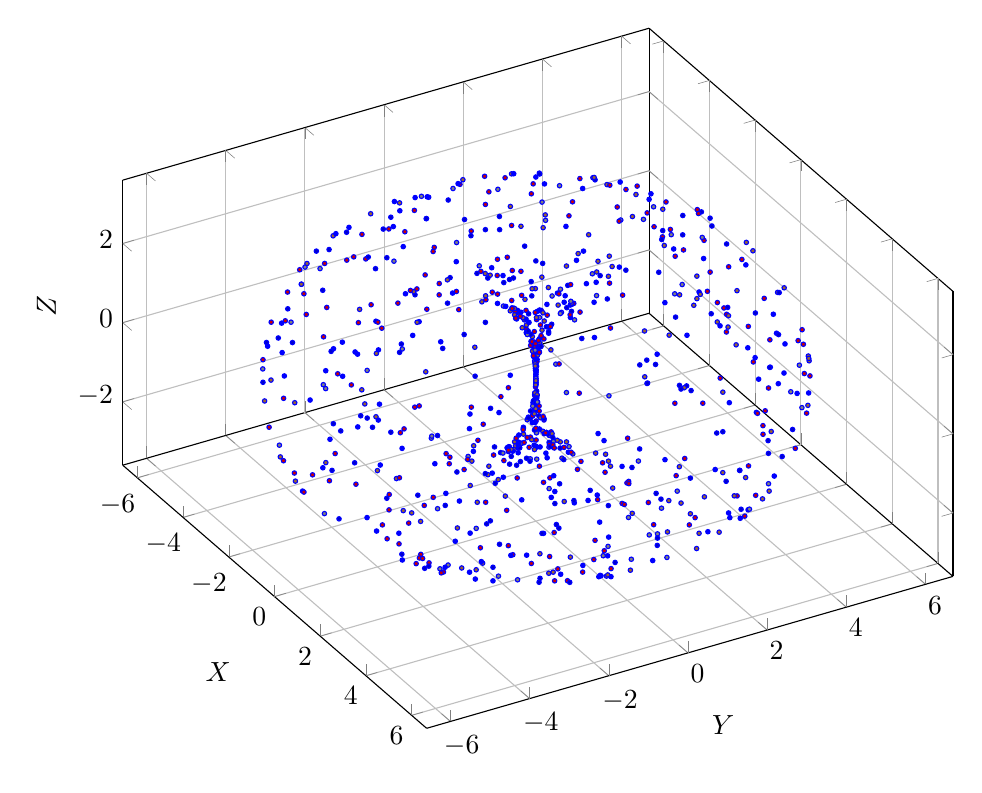
\begin{tikzpicture}
          \begin{axis}[
                view={60}{30},
                width=\textwidth, 
                axis equal,
                grid=major,
                xlabel={$X$},
                ylabel={$Y$},
                zlabel={$Z$},
        %        title={Random Points Inside a Horn Torus},
                samples=50,
                domain=0:360,
                y domain=0:360
            ]
            
            % Define parameters for a horn torus
            \pgfmathsetmacro{\R}{3}  % Major radius, set equal to minor radius
            \pgfmathsetmacro{\r}{3}  % Minor radius, set equal to major radius
            \pgfmathsetmacro{\thickness}{0.7} % Thickness to control the spread within the torus tube
        
            % Generate random points inside the horn torus
            \foreach \i in {1,...,888} {
                \pgfmathsetmacro{\theta}{random(0, 360)}
                \pgfmathsetmacro{\phi}{random(0, 360)}
                \pgfmathsetmacro{\radialDist}{\r + random(-\thickness, \thickness)}
                \pgfmathsetmacro{\x}{(\R + \radialDist * cos(\phi)) * cos(\theta)}
                \pgfmathsetmacro{\y}{(\R + \radialDist * cos(\phi)) * sin(\theta)}
                \pgfmathsetmacro{\z}{\radialDist * sin(\phi)}
        
                \addplot3+[only marks, mark=*, mark size=0.8pt, color=blue] coordinates {(\x, \y, \z)};
            }
            \end{axis}
        \end{tikzpicture}
    \caption[Horn Torus point cloud]{\textbf{Horn Torus point cloud.} Coded in to render in LaTeX with the help of ChatGPT $4$o.}
    \label{Wolfram Horn Torus}
\end{figure}
\clearpage



\section{The Data Visualisation Catalogue by Severino Ribecca}

\begin{figure}[h!]
    \centering
    \includegraphics[height=0.8\textheight]{figures/A.2.png}
    \caption[The Data Visualisation Catalogue]{\textbf{The Data Visualisation Catalogue.} 
\citep{ribecca_data_2017}. Used with Ribecca's permission.}
    \label{fig:A.2}
\end{figure}
\index[people]{Ribecca, Severino}
\clearpage

\section{Semantic Field \textit{S}}
\label{Appendix Semantic Field S}

In this section, I list the 310 terms of Semantic Field \textit{S}, as discussed in Chapter 5. To arrive at this list, I uploaded my thesis as a PDF to ChatGPT $4$o and parsed its keywords with the following prompt sequence: 
\begin{enumerate}
    \item[\textbf{1}] ``Categorize and list the key words in this document."
    \item[\textbf{2}] ``Write these as a list separated by commas, ranked by their relevance in the text"
\end{enumerate}

\rule{\linewidth}{0.4pt}


\begin{multicols}{4}
\begin{enumerate}[label=\arabic*.]
\item A Dish with One Spoon
\item abduction
\item Abundant Intelligences project
\item academic cross-pollination
\item academic knowledge management (AKM)
\item accessibility
\item Artificial General Intelligence (AGI)
\item AI energy consumption
\item algorithm
\item analogy
\item anti-oppression
\item Artificial Intelligence (AI)
\item axiological paradigms
\item biocultural memory
\item biodynamic agriculture
\item Blender
\item blind spots
\item Boundary Critique
\item capitalist extractivist economy
\item ChatGPT
\item Circle Semantic Shape
\item classification of natural forms
\item climate crisis
\item climate crisis mitigation
\item climate hyperobject
\item climate resilience
\item Carbon dioxide (CO2)
\item collaborative co-creation
\item collaborative Knowledge Production
\item colligative theory formation
\item complexity management
\item composition
\item Computational Analysis of Texts and Graphs (CATG)
\item Computational Graphesis
\item Computational Semiosis
\item conceptual gateways
\item Conceptual Graphs
\item Conceptual Networks
\item Cone Semantic Form
\item Cones of Plausibility
\item consilience
\item consilience across disciplines
\item Consilience in Knowledge Activation (CKA)
\item Consilience of Inductions
\item consolation
\item constellationary fields
\item conversational model
\item Creation-as-Research
\item Creative Presentations of Research
\item criminal justice system
\item Critical Systems Thinking (CST)
\item cybernetic mycelium
\item cybernetic rhizome
\item Cylinder Semantic Form
\item data activation
\item data hierarchy
\item data hierarchy visualization
\item data ontology modeling
\item data-information-knowledge-wisdom hierarchy (DIKW)
\item data-to-knowledge transformation
\item database of databases
\item decentralized knowledge structure
\item decomposition
\item deduction
\item degree-difference
\item Design for Health (DH)
\item Design for Sustainability Transitions (DfST)
\item Design with a Capital D
\item desolation
\item diagrammatic reasoning
\item Digital Humanities
\item dimensional addition
\item dimensionality
\item disciplinary interchange
\item discourse fields
\item domain models
\item double cone in optics
\item Double-Cone Semantic Form
\item double-diamond shape
\item eco-justice
\item ecoanthroposymbiosis
\item ecojustice
\item ecological cost of AI
\item ecologically informed AI strategy
\item Embedding Projector
\item energy resources
\item Entity-Relationship (ER) diagrams
\item environmental crisis
\item environmental degradation
\item environmental sustainability
\item epistemological diversity
\item Epistemology
\item Equity-Centered Community Design
\item Equity-Centered Community Design (ECCD)
\item ethnobotany
\item ethnoecology
\item Euclidean
\item evidence synthesis
\item filtration
\item formation and growth in morphology
\item funnel plot
\item futures cone
\item general consilience (GC)
\item Generous AI
\item geometric compositions
\item Gestalt psychology
\item gigamapping
\item glass box AI
\item Global Assortativity
\item Global Topological Synchronization (GTS)
\item GPT-3
\item GPT-4
\item graph embeddings
\item graph isomorphology
\item graph LLMs
\item graph morphology
\item graph of concepts
\item graph-based ontology models
\item graphesis
\item graphical user interface (GUI)
\item graphically structured knowledge
\item graphlet interface
\item graphlets
\item hierophanic
\item HITL (Human-in-the-Loop)
\item HITL CATG KA
\item Horn of Futures
\item Horn Torus Semantic Form
\item Human Analysis of Text and Graphs (HATG)
\item humanistic interface design
\item hyper-specialization
\item hyperlinked bibliometric graphing
\item hyperobject
\item incipit
\item Inclusive Design (ID)
\item induction
\item information design
\item information overload
\item information visualization
\item information visuospatialization
\item InfraNodus
\item interbeing
\item interdisciplinarity
\item interdisciplinary consilience
\item interdisciplinary Knowledge co-Production
\item interdisciplinary Knowledge Production
\item interdisciplinary synthesis
\item interdisciplinary topic mapping
\item Intergovernmental Panel on Climate Change (IPCC)
\item interpretable AI
\item isomorphic interbeing
\item isomorphogenesis
\item isomorphology
\item knowledge abstraction and synthesis
\item Knowledge Activation (KA)
\item knowledge design studio laboratory
\item knowledge engineering
\item knowledge graphs
\item Knowledge Management (KM)
\item Knowledge Production (KP)
\item Knowledge Production for Sustainability Transitions (KPST)
\item Knowledge Production through composition
\item Knowledge Production through visuospatial Semantic Form composition
\item Knowledge Pyramid
\item Knowledge Surfacing (KSu)
\item Knowledge Surfacing, Synthesis, Translation, and Creation(KSSTP)
\item Knowledge Synthesis (KSy)
\item Knowledge Translation (KT)
\item knowledge work platforms
\item KP quantification
\item Large Language Model (LLM)
\item logoi
\item logos of form
\item Logseq
\item Loop-line
\item Low-dimensional topology
\item ludic quality
\item major diameter
\item major radius
\item manual node placement
\item Markdown language
\item material infrastructure
\item Meru Chakra
\item meta-analysis
\item meta-language
\item meta-Systematic Combining (MSC)
\item metaphysics
\item methodological framework
\item methodological pluralism
\item middle ontology
\item minor diameter
\item minor radius
\item Mistral 7B
\item MNIST handwritten digits database
\item monocrops
\item morphology
\item moving spatial network graphs
\item multi-dimensional network graphs
\item multi-mathematical approach
\item multi-scale topological data features
\item natural resources
\item network graph
\item network graph composition
\item network graphlet
\item network subgraphs
\item networked data visualization
\item node grouping
\item Obsidian
\item Ontological Semantic Network Summaries (OSNS)
\item ontology
\item opaque AI
\item oppressive terminology
\item Oslo School of Systemic Design
\item outer diameter
\item outer radius
\item particle accelerator of ideas
\item Perceptual Artifacts Lab (PAL)
\item permaculture
\item Persistence Homology (PH)
\item Personal Knowledge Management (PKM)
\item perspective in art
\item plant-human co-evolution
\item point cloud
\item point plot heatmap
\item power relations
\item qualitative methods
\item Query Graphs
\item Query Isomorphs
\item rectangular coordinate system
\item Research-Creation
\item Research-for-Creation
\item Research-from-Creation
\item researcher grouping
\item rewilding
\item Ring Torus Semantic Form
\item Roam Research
\item Semantic Field S
\item Semantic Forms
\item semantic network mapping
\item Semantic Shapes
\item Semantic Topological Semiotics
\item simplicial complex
\item Small Language Models
\item social inequality
\item social justice
\item Social Sciences and Humanities Research Council
\item spatial and temporal modeling
\item spatial composition
\item spatial network graphs
\item spatial semiotic representation
\item spatial topic model network graphs
\item Sphere Semantic Form
\item Sri Yantra
\item stakeholder
\item Sustainability Transitions Knowledge Activation (STKA)
\item studio laboratory of knowledge design
\item surfaces of revolution
\item sustainability solutions frameworks
\item Sustainability Transitions (ST)
\item symbol composition
\item Symbol-setting
\item symbolic representation
\item syntopical consilience
\item Syntopical Consilience Abduction (SCA)
\item syntopical reading
\item Syntopicon
\item Systematic Combining (SC)
\item Systemic Design
\item Systemic Design Association (SDA)
\item Systems Oriented Design (SOD)
\item Systems Theory
\item Systems Thinking
\item Topological Capta Analysis (TCA)
\item TCA Researcher Grouping
\item TCA Workspace
\item tensors
\item Terroir of Text and Graphs (TTG)
\item text graphs
\item thought forms
\item thought signs
\item three-dimensional forms
\item three-dimensional information visualization
\item three-dimensional topic models
\item topic model network graphs
\item Topic Models
\item Topological Data Analysis (TDA)
\item Topological Capta Analysis (TCA)
\item topological semiotics
\item Topology
\item toroidal manifold
\item torus
\item transdisciplinary KA (Knowledge Activation)
\item Tree of Porphyry
\item UN Sustainable Development Goals (SDGs)
\item University
\item upper ontology
\item vector embeddings
\item vector search
\item Vedic visuospatial culture
\item visual argument
\item visual epistemology
\item visual reasoning
\item visuospatial epistemology
\item visuospatial forms of knowledge production
\item visuospatial knowledge activation interface
\item visuospatial reasoning
\item weighting
\item wicked problem
\item Zettelkasten
\item Zone of Semantic Stasis
\end{enumerate}
\end{multicols}
\clearpage

\section{Adler’s 102 \textit{Great Ideas}}
The following terms are listed alphabetically as per The \textit{Great Ideas: a Syntopicon of Great Books of the Western World} (1952), derived from the texts in \textit{Great Books of the Western World} (1952).
\begin{multicols}{4} % Use 2 or 3 columns, whichever fits well
\begin{enumerate}[label=\arabic*.]
    \item Angel
    \item Animal
    \item Aristocracy
    \item Art
    \item Astronomy and Cosmology
    \item Beauty
    \item Being
    \item Cause
    \item Chance
    \item Change
    \item Citizen
    \item Constitution
    \item Courage
    \item Custom and Convention
    \item Definition
    \item Democracy
    \item Desire
    \item Dialectic
    \item Duty
    \item Education
    \item Element
    \item Emotion
    \item Eternity
    \item Evolution
    \item Experience
    \item Family
    \item Fate
    \item Form
    \item God
    \item Good and Evil
    \item Government
    \item Habit
    \item Happiness
    \item History
    \item Honor
    \item Hypothesis
    \item Idea
    \item Immortality
    \item Induction
    \item Infinity
    \item Judgement
    \item Justice
    \item Knowledge
    \item Labor
    \item Language
    \item Law
    \item Liberty
    \item Life and Death
    \item Logic
    \item Love
    \item Man
    \item Mathematics
    \item Matter
    \item Mechanics
    \item Medicine
    \item Memory and Imagination
    \item Metaphysics
    \item Mind
    \item Monarch
    \item Nature
    \item Necessity and Contingency
    \item Oligarchy
    \item One and Many
    \item Opinion
    \item Opposition
    \item Philosophy
    \item Physics
    \item Pleasure and Pain
    \item Poetry
    \item Principle
    \item Progress
    \item Prophecy
    \item Prudence
    \item Punishment
    \item Quality
    \item Quantity
    \item Reasoning
    \item Relation
    \item Religion
    \item Revolution
    \item Rhetoric
    \item Same and Other
    \item Science
    \item Sense
    \item Sign and Symbol
    \item Sin
    \item Slavery
    \item Soul
    \item Space
    \item State
    \item Temperance
    \item Theology
    \item Time
    \item Truth
    \item Tyranny and Despotism
    \item Universal and Particular
    \item Virtue and Vice
    \item War and Peace
    \item Wealth
    \item Will
    \item Wisdom
    \item World
\end{enumerate}
\end{multicols} % Use 2 or 3 columns, whichever fits well
\clearpage


\section{Authors included in \textit{Great Books of the Western World} (1952)}
The \textit{Great Books of the Western World} (1952) includes works by the following authors:
\begin{multicols}{4}
\RaggedRight Homer\\
Aeschylus\\
Sophocles\\
Euripides\\
Aristophanes\\
Herodotus\\
Thucydides\\
Plato\\
Aristotle\\
Hippocrates\\
Galen\\
Euclid\\
Archimedes\\
Apollonius\\
Nichomachus\\
Lucretius\\
Epictetus\\
Marcus Aurelius\\
Virgil\\
Plutarch\\
Tacitus\\
Ptolemy\\
Copernicus\\
Kepler\\
Plotinus\\
Augustine\\
Thomas Aquinas\\
Dante\\
Chaucer\\
Machiavelli\\
Hobbes\\
Rabelais\\
Montaigne\\
Shakespeare\\
Gilbert\\
Galileo\\
Harvey\\
Cervantes\\
Francis Bacon\\
Descartes\\
Spinoza\\
Milton\\
Pascal\\
Newton\\
Huygens\\
Locke\\
Berkeley\\
Hume\\
Swift\\
Sterne\\
Fielding\\
Montesquieu\\
Rousseau\\
Adam Smith\\
Gibbon\\
Kant\\
J. S. Mill\\
Boswell\\
Lavoisier\\
Fourier\\
Faraday\\
Hegel\\
Goethe\\
Melville\\
Darwin\\
Marx\\
Engels\\
Tolstoy\\
Dostoyevsky\\
William James\\
Freud
\end{multicols}
\clearpage





\section{Categorizing the subjects of this thesis}
\raggedcolumns
\begin{multicols}{2}

\noindent\hangindent=1.5em \textbf{Computer Science} \\
Artificial Intelligence (AI) \\
Machine Learning \\
Natural Language Processing (NLP) \\
Computational Linguistics \\
Data Science \\
Human-Computer Interaction (HCI) \\
Information Retrieval \\
Knowledge Representation and Reasoning \\
Topological Data Analysis (TDA) \\
Graph Theory \\
\vspace{4mm}

\noindent\hangindent=1.5em \textbf{Mathematics} \\
Topology \\
Geometry \\
Computational Topology \\
Mathematical Modeling \\
\vspace{4mm}

\noindent\hangindent=1.5em \textbf{Philosophy} \\
Philosophy of Information \\
Philosophy of Language \\
Epistemology \\
Semiotics \\
Philosophy of Science \\
Ontology \\
\vspace{4mm}

\noindent\hangindent=1.5em \textbf{Cognitive Sciences} \\
Cognitive Psychology \\
Cognitive Neuroscience \\
Visual Cognition \\
Embodied Cognition \\
\vspace{4mm}

\noindent\hangindent=1.5em \textbf{Information Science} \\
Knowledge Management \\
Personal Knowledge Management (PKM) \\
Information Visualization \\
Library and Information Science \\
Ontologies \\
Digital Libraries \\
\vspace{4mm}

\noindent\hangindent=1.5em \textbf{Design} \\
Systems Oriented Design (SOD) \\
Systemic Design \\
Information Design \\
Visual Communication Design \\
Human-Centered Design \\
\vspace{4mm}

\noindent\hangindent=1.5em \textbf{Digital Humanities} \\
Computational Humanities \\
Digital Scholarship \\
Humanistic Interface Design \\
\vspace{4mm}

\noindent\hangindent=1.5em \textbf{Interdisciplinary Studies} \\
Sustainability Transitions \\
Environmental Studies \\
Climate Science \\
Ecojustice \\
Indigenous Studies \\
Decolonizing Methodologies \\
\vspace{4mm}

\noindent\hangindent=1.5em \textbf{Linguistics} \\
\RaggedRight Computational Linguistics \\
Semantics \\
Pragmatics \\
Language and Thought \\
\vspace{4mm}

\noindent\hangindent=1.5em \textbf{Education} \\
Knowledge Activation \\
Collaborative Learning \\
\RaggedRight Interdisciplinary Education \\
Educational Technology \\
\vspace{4mm}

\noindent\hangindent=1.5em \textbf{Sociology} \\
Sociology of Knowledge \\
Science and Technology Studies (STS) \\
Cultural Studies \\
\vspace{4mm}

\noindent\hangindent=1.5em \textbf{Communication Studies} \\
Media Studies \\
Information Theory \\
Symbolic Communication \\
\vspace{4mm}

\noindent\hangindent=1.5em \textbf{Ethnography and Anthropology} \\
Ethnoecology \\
Ethnobotany \\
Cultural Anthropology \\
\vspace{4mm}

\noindent\hangindent=1.5em \textbf{Visual Studies} \\
Visual Epistemology \\
Visual Reasoning \\
Visual Semiotics \\
Graphical Representation \\
\end{multicols}

\clearpage






\section{Experts consulted}
I acknowledge with professional admiration the subject matter experts who provided formative feedback for this thesis. I list their names here in alphabetical order by surname:

\begin{itemize}[label={}]
    \item \textbf{Dr. Evan Timothy Barba}, Associate Professor at Georgetown University
    \item \textbf{Tega Brain}, artist and Associate Professor at New York University (NYU)
    \item \textbf{Antionette D. Carroll}, founder of the Institute of Equitable Design and Justice, and Creative Reaction Labs
    \item \textbf{John P. Comer}, founder of Architects Of Justice; National Organizing Director of The Redress Movement
    \item \textbf{Dr.Peter Coppin}, Director of the The Perceptual Artifacts Lab (PAL) and  Associate Professor of Design at OCAD University. 
    \item \textbf{Dr. Sara Diamond}, OCAD University Research Chair, Director of the Visual Analytics Lab, and Co-investigator of the OCAD U Abundant Intelligences A Dish with One Spoon – Towards “Generous AI” Invention and Collaboration project
    \item \textbf{Dr. Michael Doser}, senior research physicist at the European Council for Nuclear Research/Conseil Européen pour la Recherche Nucléaire (CERN)
    \item \textbf{Balazs Farago}, founder and CEO of Walters Cube.
    \item \textbf{Ekaterina Grgurić}, Digital Scholarship Librarian at the University of British Columbia (UBC)
    \item \textbf{Michael Groenendyk}, Digital Scholarship Librarian at Concordia University
    \item \textbf{Micki Kaufman}, historian and digital scholar at the City University of New York
    \item \textbf{Dr. Peter Jones}, founder of the Strategic Innovation Lab, co-founder of the Systemic Design Association, and Distinguished Professor in Systemic Design for the School of Architecture, Art and Design at the Tecnológico de Monterrey
    \item \textbf{Amanda Licastro}, Digital Scholarship Librarian at Swarthmore College
    \item \textbf{Dr. Blake Madill}, Associate Professor of Pure Mathematics at the University of Waterloo
    \item \textbf{Cheryl May}, Executive Editor for the Systemic Design Association, and PhD candidate at London South Bank University
    \item \textbf{Dr. Gavin Mendel-Gleason}, CTO of TerminusDB, and former research fellow at Trinity College Dublin in the School of Statistics and Computer Science
    \item \textbf{Ola Mazzuca}, exhibition operations at the Gallery at Mason Studio
    \item \textbf{Antonio Muñoz Gomez}, Digital Scholarship Librarian at the University of Waterloo
    \item \textbf{Dr. Lennart Nacke}, University Research Chair and Professor at the University of Waterloo, and Associate Director of the Stratford School of Interaction Design and Business, and Director of the HCI Games Group at the University of Waterloo's Games Institute
    \item \textbf{Rahul Nayak}, data scientist from the Indian Institute of Technology
    \item \textbf{Dr. Dmitry Paranyushkin}, founder of InfraNodus and senior researcher at Nodus Labs
    \item \textbf{Dr. Paul Pangaro}, President of the American Society for Cybernetics
    \item \textbf{Dr. Michael J. Prokopow}, cultural historian, curator, and professor at OCAD University
    \item \textbf{Santiago Ortiz}, director of Moebio Labs
    \item \textbf{Ryan J. A. Murphy}, PhD candidate at the University of Newfoundland and Co-Secretary of the Systemic Design Association
    \item \textbf{Dr. Birger Sevaldson}, professor at the Oslo School of Architecture and Design, and at the University of South-Eastern Norway
    \item \textbf{Peter Scott}, lecturer at OCAD University
    \item \textbf{Dr. Maria Aleksandrovna Simakova}, Foucault scholar from the University of Toronto
    \item \textbf{Kirsta Stapelfeldt}, Associate Librarian, Research and Digital Initiatives at the University of Toronto Scarborough Digital Scholarship Unit
    \item \textbf{Brian Sunter}, software engineer from the University of Florida
    \item \textbf{Serkan Özkaya}, conceptual artist
    \item \textbf{David Kwasny}, Data and Digital Literacy Librarian at the University of Toronto Scarborough Digital Scholarship Unit
    \item \textbf{Kyle Winters}, CEO of NEXT Canada
\end{itemize}

\clearpage






\section{Research presentations}

In this section, I list the presentations I delivered about my work during my thesis research: \\

\begin{enumerate}


    \item[{2024}] \textit{Systems Oriented Disruptions}, presented for the annual International Innovation Forum hosted by the Strategic Foresight and Innovation program in the OCAD University School of Graduate Studies
 
    \item[{2024}] \textit{Systems Oriented Disruptions}, presented for Creative Disruptions// re-imagining our futures the graduate thesis exhibition by the Digital Futures program in the OCAD University’s School of Graduate Studies

    \item[{2024}]  \textit{Body of Aesthetics}, a panel discussion moderated by curator Sara Dagovic and joined by artist Artemis Han, The Gallery at Mason Studio, Toronto

    \item[{2023}] \textit{Three-dimensional plotting of information categories using P5.js}, Perceptual Artifacts Lab in OCAD University, moderated by the PAL Director Dr. Peter Coppin  

    \item[{2023}] \textit{Song Within a Sacrifice Zone}, presented for \textit{Uses and Abuses of Power in Alternative Spiritualities}, the annual conference by the Program for the Evolution of Spirituality in the Harvard Divinity School
 
    \item[{2023}] \textit{The biopower of faith leaders who are also alternative medicine practitioners in alternative spiritual communities}, presented for \textit{Uses and Abuses of Power in Alternative Spiritualities}, the annual conference by the Program for the Evolution of Spirituality in the Harvard Divinity School
 
    \item[{2023}] \textit{Knowledge Translation vs the Climate Crisis} presented for the annual colloquium hosted by the Digital Futures in the OCAD University School of Graduate Studies
 
    \item[{2022}] \textit{Dissonance}, presented for the Too Big To Fail Exhibition organized by the Interdisciplinary Master’s of Art, Media and Design in the OCAD University School of Graduate Studies

    \item[{2022}] \textit{Data Tori}, presented for the annual Graduate Colloquium, moderated by Duchamp scholar Dr. Julian Haladyn, in the OCAD University School of Graduate Studies

    \item[{2022}] \textit{Medicinallity of Symbol}, presented for the annual research panel organized by the Interdisciplinary Master’s of Art, Media and Design, in the OCAD University School of Graduate Studies, moderated by Graduate Program Director Jay Irizawa
    
\end{enumerate}
\clearpage




\section{Art exhibitions}

In this section, I list the art exhibitions in which I showcased my work during my thesis research: \\

\begin{enumerate}
    \item[{2024}] \textit{GradEx 109}, OCAD University

    \item[{2024}] \textit{Creative Disruptions// re-imagining our futures}, Digital Futures graduate thesis exhibition, OCAD University, Waterfront Campus. 
 
    \item[{2024}] \textit{Body of Aesthetics, curated by Sara Dagovic}, The Gallery at Mason Studio, Toronto

    \item[{2023}] \textit{Digital Futures Open Show}, OCAD University, School of Graduate Studies

    \item[{2023}] \textit{Song Within a Sacrifice Zone}, Harvard Divinity School, Swartz Hall
 
    \item[{2023}] \textit{Resilience and Connection: artistic explorations of mental health}, L.R. Wilson Building, McMaster University 
 
    \item[{2023}] \textit{Too Big to Fail}, Open Space Gallery, OCADU
 
    \item[{2022}] \textit{The Incomplete}, The Great Hall Gallery, OCADU
\end{enumerate}
\clearpage





\section{Resources and tools tested and used during thesis}
\label{Appendix Resources and Tools}
\begin{multicols}{2}

\noindent\hangindent=1.5em \textbf{Hardware} \\
Macbook Pro, 16-inch, 2021, Apple M1 Max, 32 GB RAM

\vspace{4mm}

\noindent\hangindent=1.5em \textbf{Source Management} \\
Zotero \\
\RaggedRight \hangindent=1.5em Zotero Better BibTex extension v 6.7.202 by Emiliano Heyns (to generate citation keys) \\
Zotero Connector Chrome extension \\

\vspace{4mm}

\noindent\hangindent=1.5em \textbf{Personal Knowledge Management (PKM)} \\
Obsidian \\
Logseq \\
Logseq PDF reader \\
Readwise Official Plugin v1.4.9 \\
Roam Research \\
\vspace{4mm}
\noindent\hangindent=1.5em \textbf{Three-Dimensional Forms} \\
Blender, node programming \\

\vspace{4mm}

\noindent\hangindent=1.5em \textbf{Document Drafting} \\
\RaggedRight \hangindent=1.5em Overleaf, Online LaTeX editor \\
\RaggedRight \hangindent=1.5em Dissertate, LaTeX dissertation template by Jordan Suchow \\
\RaggedRight \hangindent=1.5em Pandoc for populating Better BibTeX citation keys into in-sentence citation and list of references \\
Google Docs \\
Google Chrome extension DocsAfter Dark \\
Microsoft Word \\

\vspace{4mm}

\noindent\hangindent=1.5em \textbf{Document Reading} \\
Zotero PDF reader \\
ProQuest Ebook Central \\
The Internet Archive \\
Logseq PDF reader \\
Readwise \\
Readwise Reader \\
\RaggedRight \hangindent=1.5em Readwise Chrome extension (synced to Logseq and Obsidian) \\
Apple Photos Optical Character Recognition \\
Adobe Acrobat \\
Adobe Digital Editions \\

\vspace{4mm}

\noindent\hangindent=1.5em \textbf{Infinite Canvas Text Analysis Tools} \\
Miro \\
Scapple \\

\vspace{4mm}

\noindent\hangindent=1.5em \textbf{Text Graphing Tools} \\
InfraNodus \\
\RaggedRight \hangindent=1.5em InfraNodus Chrome extension for its 3D knowledge graph \\
MIT’s SIMILE Timeline widget, run on Zotero \\
Obsidian Canvas, core plugin \\ 
Obsidian Outline, core plugin \\
Obsidian Graph View, core plugin \\
\RaggedRight \hangindent=1.5em Obsidian 3D Graph v1.0.5, community plugin by Alexander Weichart \\
Python 3.8.12 \\
PiVis* \\
Pandas Dataframes* \\
NetworkX* \\
Voyant Tools \\
* Python libraries \\

\vspace{4mm}


\noindent\hangindent=1.5em \textbf{LLMs} \\
Mistral 7B Open Orca* \\
Zephyr* \\
Grammarly AI Writing Assistant \\
Claude 3.5 Sonnet \\
Google Gemini Advanced 1.5 Pro\\
Chat GPT 3.5 \\
Chat GPT 4 \\
Chat GPT 4 Turbo \\
Chat GPT $4$o \\
Chat GPT 4-mini \\
Chat GPT o1-preview \\
Chat GPT o1 \\
Chat GPT o1-mini \\
* set up using Ollama \\

\vspace{4mm}


\noindent\hangindent=1.5em \textbf{Image Management} \\
Apple Photos \\
Affinity \\
Affinity Designer \\
Affinity Publisher \\
Pinterest \\
QuickTime Player \\

\vspace{4mm}

\noindent\hangindent=1.5em \textbf{Audio and Video Production} \\
\RaggedRight Final Cut Pro \\ 
\RaggedRight Logic Pro \\

\vspace{4mm}

\noindent\hangindent=1.5em \textbf{Typefaces in Figures} \\
iA Writer Quattro S \\
Helvetica Neue \\
Arial Black \\
Avenir Next Condensed \\

\vspace{4mm}

\noindent\hangindent=1.5em \textbf{Typefaces in Document} \\
Lato - used for text captions \\
Noto Mono - used for code \\
EB Garramond - used for all other text \\

\end{multicols}

\clearpage

%\chapter*{Indices}
%\addcontentsline{toc}{chapter}{Indices}
%\label{Index}



